\subsection{Descoberta de Serviços em Ambientes de TVDI \cite{borges2007arquitetura}} 

Um ambiente de TV Digital Interativa (TVDI)\nomenclature{TVDI}{TV Digital Interativa} pode oferecer, aos seus usuários, uma grande quantidade de serviços. Tais serviços podem ser acessados pelo Guia Eletrônico de Programação (\textit{Eletronic Program Guide}, EPG \nomenclature{EPG}{\textit{Eletronic Program Guide}}). No entanto, muitos outros serviços podem ser disponibilizados por meio do acesso ao canal de retorno, que não são catalogados pelo EPG. Tecnologias como Jini, \textit{Service Location Protocol} e \textit{Universal Plug and Play} podem ser utilizadas para descoberta de serviços em infra-estruturas híbridas como a de TVDI. Elas permitem que os usuários tomem conhecimento dos serviços que lhe são disponibilizados.

Tendo em vista as diferentes tecnologias existentes, em \cite{borges2007arquitetura} é apresentada uma proposta para possibilitar o uso transparente, independente de localização, de serviços providos por diferentes protocolos de descoberta. É apresentada uma arquitetura, a ser incorporada no middleware dos receptores de TVD\nomenclature{TVD}{TV Digital}.

\subsubsection{Protocolos de Descoberta de Serviços} \label{service-discovery-protocols}

Protocolos para descoberta dinâmica de serviços tem sido criados para liberar o usuário da necessidade de conhecer o endereço do serviço e efetuar configurações para utilizá-lo. Sistemas para descoberta permitem que sejam divulgados serviços, sendo que os clientes podem buscar tais serviços com base em seus atributos publicados.

Arquiteturas existentes para descoberta de serviços são compostas, de pelo menos, dois elementos: os provedores de serviços e os usuários de serviços. Em algumas arquiteturas existe um elemento intermediário, responsável por gerenciar os serviços, como em \cite{al2008toward}. Em sistemas sem um gerenciador, as requisições dos usuários são enviadas diretamente aos provedores. Em sistemas com gerenciador, inicialmente os provedores registram seus serviços no gerenciador, e/ou este varre a Web em busca de serviços públicos, como em \cite{al2008toward}.

%\subsubsubsection{Jini}
\textbf{Jini}

O projeto Jini, inicialmente desenvolvido pela \textit{Sun Microsystems}, atualmente suportado pela \textit{Apache Software Foundation} e denominado \textit{Apache River}, é uma arquitetura orientada a serviços, que define um modelo de programação, que explora e estende a tecnologia Java, para habilitar a construção de sistemas distribuídos seguros, consistindo de federações de serviços e clientes. A tecnologia Jini também pode ser usada para construir sistemas de rede adaptativos, escaláveis, evolutívos e flexíveis, como tipicamente requerido em ambientes de computação dinâmica \cite{apache-river}.

A arquitetura Jini é desenvolvida em linguagem Java e utiliza o modelo de objetos distribuídos \textit{Remote Method Invocation} (RMI)\nomenclature{RMI}{\textit{Remote Method Invocation}} e possibilita que as referências dos objetos remotos sejam carregadas entre receptores com a \textit{Java Virtual Machine} (JVM)\nomenclature{JVM}{\textit{Java Virtual Machine}}. Ela possui ainda um sistema de alerta sobre a disponibilidade de serviços buscados pelo usuário.

A Figura \ref{fig:jini-sequence-diagram} apresenta um diagrama de sequências, mostrando algumas mensagens trocadas na interação entre os componentes da arquitetura Jini.

\begin{center}
	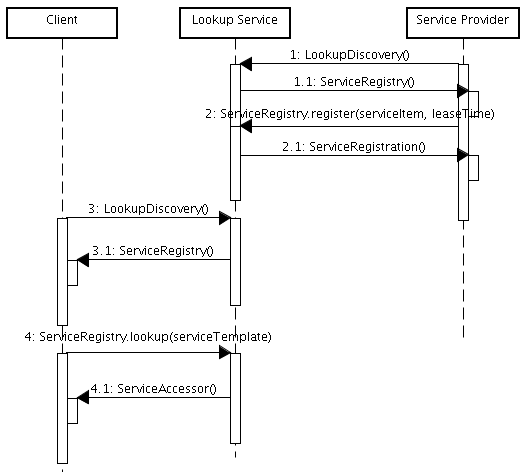
\includegraphics[scale=0.6]{images/jini-sequence-diagram.png}
	\captionof{figure}{Diagrama de sequência para componentes Jini (adaptada de \cite{borges2007arquitetura}).}
	\label{fig:jini-sequence-diagram}
\end{center}

Tanto os clientes quanto os provedores de serviços precisam descobrir o endereço do \textit{Lookup Service}, enviando uma mensagem \textit{multicast} (\textit{LookupDiscovery}) para localizar este servidor. O \textit{Lookup Service} é responsável por gerenciar os serviços de diferentes provedores, interligando os clientes a estes.
Os provedores de serviço devem registrar seus serviços junto ao \textit{Lookup Service} (\textit{ServiceRegistry.register}), para que os clientes possam utilizar tais serviços. E por fim, os clientes podem buscar por um determinado serviço (\textit{ServiceRegistry.lookup}), baseado em critérios definidos por ele.

%\subsubsubsection{\textit{Service Location Protocol} (SLP)}
\textbf{\textit{Service Location Protocol} (SLP)}

O protocolo SLP\nomenclature{SLP}{\textit{Service Location Protocol}} foi desenvolvido pelo \textit{Internet Engineering Task Force} (IETF) \nomenclature{IETF}{\textit{Internet Engineering Task Force}} para permitir a descoberta de serviços, sem que os clientes necessitem conhecer sua localização \cite{borges2007arquitetura}. Também baseado em uma arquitetura de 3 camadas, como o Jini, sendo seus elementos:

\begin{itemize}
	\item \textit{User Agents} (UA): cliente que realiza a busca por serviços;
  \item \textit{Service Agents} (SA): anuncia e controla os serviços por ele disponibilizados (equivalente ao \textit{Service Provider} na arquitetura Jini);
  \item \textit{Directory Agents}: mantém uma lista dos serviços nele registrados, intermediando as interações entre os UAs e os SAs (equivalente ao \textit{Lookup Service} na arquitetura Jini).
\end{itemize}

A troca de mensagens usando o protocolo SLP também é semelhante ao que ocorre na arquitetura Jini, como pode ser visto na Figura \ref{fig:slp-flow-message}.

\begin{center}
	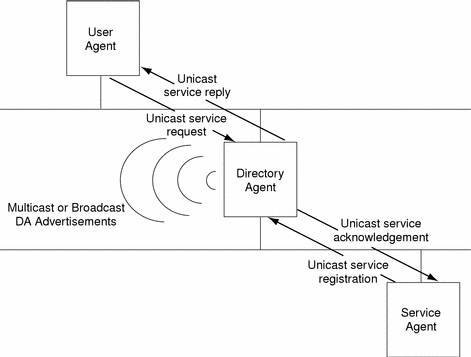
\includegraphics[width=0.7\textwidth]{images/slp-flow-message.png}
	\captionof{figure}{Troca de mensagens entre componentes do protocolo SLP \cite{slp-admin-guide}}
	\label{fig:slp-flow-message}
\end{center}

%\subsubsubsection{Universal Plug and Play (UPnP)}
\textbf{Universal Plug and Play (UPnP)}

O UPnP\nomenclature{UPnP}{\textit{Universal Plug and Play}} é um conjunto de protocolos para descoberta de serviços, desenvolvido por um consórcio de empresas, liberado pela \textit{Microsoft}. Ele define uma arquitetura para estender o modelo de periféricos \textit{Microsoft Plug and Play}, visando um modelo altamente dinâmico para a integração com vários dispositivos de redes de diferentes fabricantes \cite{borges2007arquitetura}. A arquitetura UPnP define protocolos de comunicação entre controladores e dispositivos, para descoberta, descrição, controle, eventos e apresentação, sendo eles: \textit{Simple Service Discovery Protocol} (SSDP), \textit{General Event Notification Architecture} (GENA), SOAP, HTTP, XML, TCP/IP e UDP \cite{borges2007arquitetura}. Um grande ponto forte do protocolo é a utilização de padrões como HTTP, XML e SOAP, permitindo que a troca de mensagens seja feita utilizando protocolos Web padronizados, o que evita problemas com portas bloqueadas em \textit{Firewalls}.

%\subsubsubsection{\textit{Service Discovery Protocol} (SDP)}
\textbf{\textit{Service Discovery Protocol} (SDP)}

O SDP\nomenclature{SDP}{\textit{Service Discovery Protocol}} faz parte das especificações \textit{Bluetooth} (IEEE 802.15.1), e é utilizado para descoberta de serviços em uma \textit{Personal Area Network} (PAN)\nomenclature{PAN}{\textit{Personal Area Network}}, sendo uma arquitetura de duas camadas, contendo dois agentes: o \textit{SDP Server} e o \textit{SDP Client}. 

\subsubsection{Solução Proposta}

Em \cite{borges2007arquitetura} é apresentada uma arquitetura para descoberta de serviços em ambientes de TVDI. O trabalho cita um caso de uso de uma pizzaria que deseja fazer uma promoção pela TVD, por um determinado período de tempo. A aplicação deve ser disponibilizada via \textit{broadcast} para seus usuários e a promoção deve durar um tempo determinado. Como o total de usuários que venham a utilizar a aplicação pode ser alto, isto pode sobrecarregar o serviço. Desta forma, é necessário um mecanismo de balanceamento de carga para distribuir os pedidos de pizza entre as diversas filiais da rede de pizzarias que promoveu a promoção, onde cada filial estaria provendo o serviço de pedidos de pizza pela TVDI. Além disto, \cite{borges2007arquitetura} cita que a aplicação pode estar disponível para usuários com dispositivos móveis. Desta forma, é necessário que a descoberta de serviços, disponíveis na localidade atual do usuário, seja feita sem a necessidade de configurações manuais.

O trabalho em \cite{borges2007arquitetura} apresenta uma proposta de arquitetura para descoberta de serviços em TVDI, que contempla os requisitos citados anteriormente.

%\subsubsubsection{Arquitetura da Solução}
\textbf{Arquitetura da Solução}

A arquitetura proposta em \cite{borges2007arquitetura} é composta por três camadas, descritas a seguir.

\begin{itemize}
	\item Aplicações: camada contendo as aplicações clientes executados no receptor digital (fixo, móvel ou portátil).
  \item \textit{Middleware}: encapsula os componentes para busca, atualização e registro de serviços, além das funcionalidades de tempo de disponibilização dos serviços e balanceamento de carga.
  \item Protocolos de Descoberta de Serviços: infra-estrutura para acesso aos diversos protocolos de descoberta de serviços, tratados na Seção \ref{service-discovery-protocols}.
\end{itemize}

A Figura \ref{fig:arq-descoberta-servicos-tvdi} apresenta a arquitetura da solução apresentada em \cite{borges2007arquitetura}.

O tipo de protocolo de descoberta de serviços é irrelevante para a aplicação. Para tornar este acesso transparente, foram desenvolvidos componentes no \textit{middleware}, que são acessados pela aplicação, a partir de uma API desenvolvida. O acesso aos diferentes protocolos de descoberta pode ser feito por meio de um canal de retorno.

Os componentes implementados, que devem estar presentes na camada de \textit{middleware}, sendo incorporados a ele, são definidos a seguir.

\begin{itemize}
	\item Busca: possibilita a busca de serviços disponibilizados para o ambiente de TVDI, independente do protocolo de descoberta subjacente.
  \item Registro: possibilita que um usuário disponibilize serviços armazenados em seu receptor digital, a outros usuários.
  \item Atualização: possibilita que altere ou torne indisponível um serviço.
  \item Temporalidade: permite definir um período de tempo no qual o serviço estará disponível.
  \item Balanceamento: permite balancear a carga de acessos a um determinado serviço, para diferentes provedores do mesmo serviço.
\end{itemize}

\begin{center}
	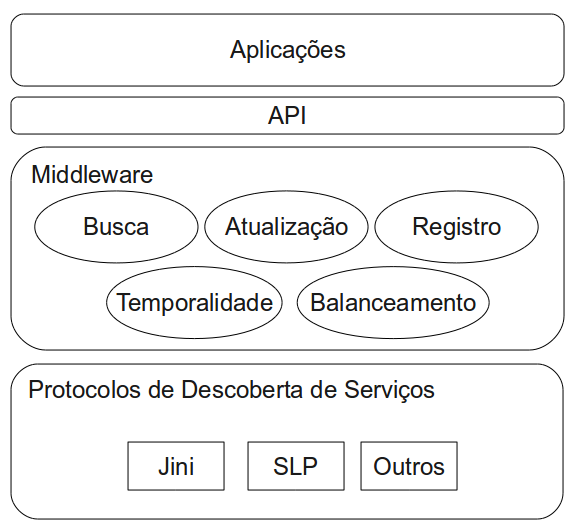
\includegraphics[width=0.70\textwidth]{images/arquitetura-descoberta-servicos-tvdi.png}
	\captionof{figure}{Arquitetura para Descoberta de Serviços em TVDI \cite{borges2007arquitetura}}
	\label{fig:arq-descoberta-servicos-tvdi}
\end{center}

\subsubsection{Conclusões}

A arquitetura apresentada em \cite{borges2007arquitetura} permite a descoberta de serviços em ambientes de TVDI, tornando transparente para as aplicações, o tipo de protocolo de descoberta utilizado. A arquitetura é baseada em três camadas, como convencionalmente encontrado em outras propostas citadas, e possui recursos importantes como balanceamento de carga e opção para definir o tempo de disponibilidade dos serviços. Um recurso bastante interessante é a possibilidade de tornar conversores digitais de usuários em provedores de serviços, utilizando uma infra-estrutura já existente para fornecer serviços, podendo estes serem replicados em diferentes conversores, permitindo o balanceamento de carga entre eles.
